\documentclass{article}

\usepackage{microtype}
\usepackage{graphicx}
\usepackage{booktabs}
\usepackage{hyperref}
\usepackage{amsmath}
\newcommand{\theHalgorithm}{\arabic{algorithm}}
\usepackage{icml2026}
\icmltitlerunning{Evidence Before Improvement}

\begin{document}

\twocolumn[
  \icmltitle{Evidence Before Improvement: A White-Box Contract Audit for Autonomous MLIP Research}
  \begin{icmlauthorlist}
    \icmlauthor{Anonymous Author(s)}{anon}
  \end{icmlauthorlist}
  \icmlaffiliation{anon}{Anonymous Institution}
  \icmlcorrespondingauthor{Anonymous Author(s)}{anonymous@example.invalid}
  \icmlkeywords{AI scientist, interatomic potentials, reproducibility, provenance, fault injection}
  \vskip 0.3in
]
\printAffiliationsAndNotice{}

\begin{abstract}
Autonomous research agents can optimize a reported metric while silently losing the evidence needed to justify the result. We preregister a deterministic white-box contract-coverage audit of an artifact-bound research trace for machine-learning interatomic potentials (MLIPs). Twelve hand-authored fault operators were each applied to four trace instantiations, yielding 48 single-fault cases and four clean controls. The semantic grader detected 48/48 declared corruptions with no clean rejection; a mutable manifest-only integrity ablation detected 4/48. A separate, previously verified two-iteration MACE replay on an NVIDIA L4 illustrates the policy consequence: one candidate crossed the frozen metric-improvement threshold but remained rejected after its exact-equality reproducibility gate failed. These observations support an infrastructure claim about coverage of the tested contract and fault catalog, not general grader robustness, improved MACE performance, or scientific validity.
\end{abstract}

\section{Introduction}

Language-model agents can plan, execute, and write machine-learning experiments \cite{huang2024mlagentbench,yamada2025aiscientistv2}, while recent benchmarks evaluate whether agents can reproduce research artifacts \cite{starace2025paperbench}. Success metrics alone, however, do not establish that an experimental conclusion is reproducible: reproducible code and reproducible findings are distinct goals \cite{bouthillier2019reproducible}. This distinction is acute for MLIPs, where model identity, energy and force units, data partitions, hardware, and validation protocols all affect interpretation \cite{batatia2022mace,maxson2024reporting}.

We study a narrower question: \emph{does semantic re-derivation detect repository-defined trace faults more completely than producer-declared hashes?} Drawing on fault injection as a controlled dependability-analysis technique \cite{hsueh1997fault}, our contribution is a preregistered white-box contract audit over 12 fault families and four seeds, paired with a real-MACE negative-result case study. The paper intentionally stops at an infrastructure claim ceiling.

\begin{figure*}[t]
  \centering
  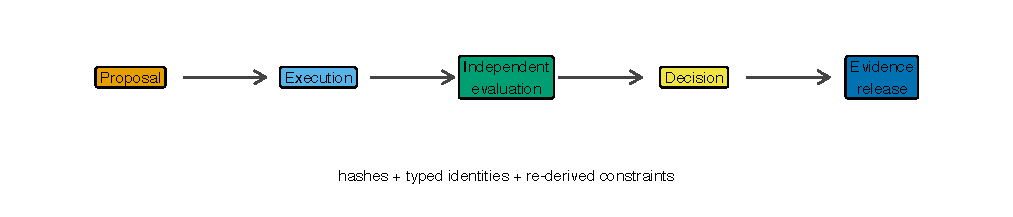
\includegraphics[width=\textwidth]{figures/evidence_workflow.pdf}
  \caption{The evaluated workflow binds proposal, execution, independent evaluation, decision, and evidence release. The semantic grader checks both artifact integrity and cross-stage constraints; agent prose and Tea Time reflection are excluded from evidence.}
  \label{fig:workflow}
\end{figure*}

\section{Method and Agent Workflow}

\paragraph{Evidence contract.}
The controller emits sealed objective, proposal, legality, execution, evaluation, decision, lesson, lineage, and manifest artifacts. The evaluator has a distinct code identity, and the decision is recomputed from frozen acceptance constraints. Reflection and reviewer text may influence a later proposal but cannot support a numerical claim. This follows the broader principle of falsification-oriented automated analysis \cite{huang2025popper}, but our grader is deterministic and does not use an LLM.

\section{Experimental Protocol}

\paragraph{Preregistered comparison.}
For each seed from 20260712--20260715, we generated one clean two-iteration synthetic trace and then made twelve separate derived copies. Each copy received exactly one frozen fault: missing Tea Time, missing lesson, evaluator identity collision, immutable-input change, forbidden label payload, unauthorized remote attestation, decision--metric inconsistency, internal-seal tamper, registered-artifact corruption, inflated scientific status, forged rejection without rollback, or broken lineage parent. The recorded execution evaluated every seed--fault pair once and reports \texttt{retry\_count=0}. The integrity ablation verifies every path, size, and SHA-256 declared in a mutable producer manifest. For semantic forgeries, that manifest is refreshed intentionally; hashes prove byte identity, not whether the bytes describe a legal experiment. The candidate additionally re-derives cross-artifact constraints.

The primary endpoint is macro fault-detection recall. Success required recall $\geq0.90$, no rejection of a clean trace, and an absolute recall gain $\geq0.25$. The benchmark used local CPU only and accessed no scientific labels, protected partitions, acquisition labels, or remote resources.

\section{Results}

\begin{figure}[t]
  \centering
  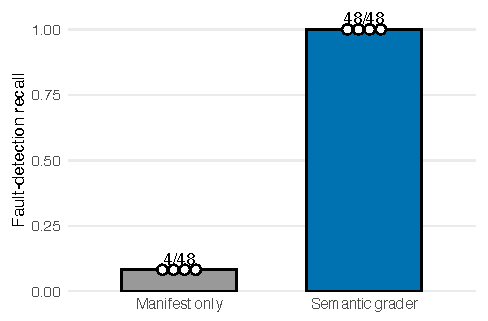
\includegraphics[width=\columnwidth]{figures/fault_detection_recall.pdf}
  \caption{Fault-detection recall over 48 preregistered corrupt traces (four seed-level points per method; 12 families per seed). Bars show aggregate exact counts, and no uncertainty bars are drawn because the finite catalog is reported without population inference. Both methods accepted all four clean controls.}
  \label{fig:recall}
\end{figure}

The semantic grader detected 48/48 corruptions (macro and micro recall 1.00) and accepted 4/4 clean controls. The manifest-only integrity ablation detected 4/48 (macro and micro recall 0.083), for a preregistered macro-recall gain of 0.917 (Table~\ref{tab:audit}); macro and micro values coincide because every family has four cases. Every threshold was met. No clean rejection was observed in four controls, which is not a precise estimate of a population false-positive rate. Because the faults were white-box and repository-defined, the result demonstrates coverage of this contract, not robustness to arbitrary attacks.

\begin{table}[t]
  \caption{Frozen fault-injection result.}
  \label{tab:audit}
  \centering
  \small
  \begin{tabular}{lccc}
    \toprule
    Method & Detected & Recall & Clean rejected \\
    \midrule
    Manifest hashes & 4/48 & 0.083 & 0/4 \\
    Semantic grader & 48/48 & 1.000 & 0/4 \\
    \bottomrule
  \end{tabular}
\end{table}

\paragraph{Real-MACE negative case.}
We also reused a hash-verified, policy-attested exact-commit replay on one NVIDIA L4. It used \texttt{mace-torch} 0.3.16, a candidate-only checkpoint, a bounded approved label view, one optimizer step per iteration, and an independent aggregate evaluator. For validation force-component MAE in $\mathrm{eV\,\mathring{A}^{-1}}$, iteration 1 improved by 0.053\%, below the frozen 0.1\% threshold, and was rejected. Iteration 2 improved by 0.133\% and passed the metric threshold, but both iterations had \texttt{rerun\_metric\_delta}=1.0 and failed the exact-equality reproducibility constraint, so both were rejected. Here 1.0 is a binary mismatch indicator, not the physical magnitude of numerical drift. Exact equality is especially conservative because numerical reproducibility can vary across software releases, platforms, and CPU/GPU execution even with identical seeds \cite{pytorch2026reproducibility}. The completed trace remained \texttt{infrastructure\_only} and claim-ineligible.

This case demonstrates the policy consequence: a metric-only rule would have promoted iteration 2, whereas the frozen multi-constraint rule retained the negative result. It does not show that the candidate was scientifically worse, because the current binary rerun endpoint cannot distinguish harmless floating-point variation from decision-relevant instability.

\section{Limitations and Conclusion}

Our fault operators were written against the grader contract, so perfect recall may overestimate coverage of unanticipated corruption. Four clean controls do not tightly bound false-positive probability. The mutable manifest-only integrity ablation is deliberately narrow, and the experiment evaluates trace validity rather than scientific truth. The MACE replay contains two infrastructure iterations on one device and no frozen-test release, physical-property validation, independent provider replication, or approved checkpoint promotion. Repeated validation access can also create adaptive bias \cite{dwork2015holdout}; this campaign makes no claim about that risk.

Within these limits, the experiment supports one conclusion: for the twelve preregistered fault families, semantic re-derivation caught failures that producer-declared hashes usually could not, without rejecting the clean controls. In the accompanying MACE case, the same fail-closed posture preserved a nominal metric improvement as a rejection rather than converting it into an unsupported performance claim. Future work should replace the binary rerun flag with tolerance-aware, decision-calibrated deltas and evaluate externally designed faults.

\bibliography{references}
\bibliographystyle{icml2026}

\end{document}
